\documentclass[11pt]{article}
\usepackage{graphicx}
\usepackage{amssymb}
\usepackage{amsmath}
\usepackage{epstopdf}
\DeclareGraphicsRule{.tif}{png}{.png}{`convert #1 `dirname #1`/`basename #1 .tif`.png}

\textwidth = 6.5 in
\textheight = 9 in
\oddsidemargin = 0.0 in
\evensidemargin = 0.0 in
\topmargin = 0.0 in
\headheight = 0.0 in
\headsep = 0.0 in
\parskip = 0.2in
\parindent = 0.0in

\newtheorem{theorem}{Theorem}
\newtheorem{corollary}[theorem]{Corollary}
\newtheorem{definition}{Definition}

\newcommand{\cut}[1]{}

\title{Matrix Calculus Jumpstart}
\author{Terence Parr and Jeremy Howard}
\begin{document}
\maketitle

\section{Introduction}

Most of us last saw calculus in school, but function derivatives are a critical part of machine learning, particularly deep learning neural networks where we optimize loss functions to train models. Pick up a machine learning paper or the documentation of a library such as PyTorch and calculus comes screeching back into your life like distant relatives around the holidays.  And it's not just any old scalar differential calculus that pops up---we need {\em matrix calculus}. 

For example, the output function of an artificial neuron (with rectified linear activation function) is typically described using a dot product  (from linear algebra) of an edge weight vector $\mathbf{w}$ with an input vector $\mathbf{x}$ plus a scalar bias (threshold): $output(\mathbf{x}) = max(0, \Sigma_i^n w_i x_i + b) = max(0, \mathbf{w} \cdot \mathbf{x} + b)$. Visually that neuron looks like:

\begin{center}
	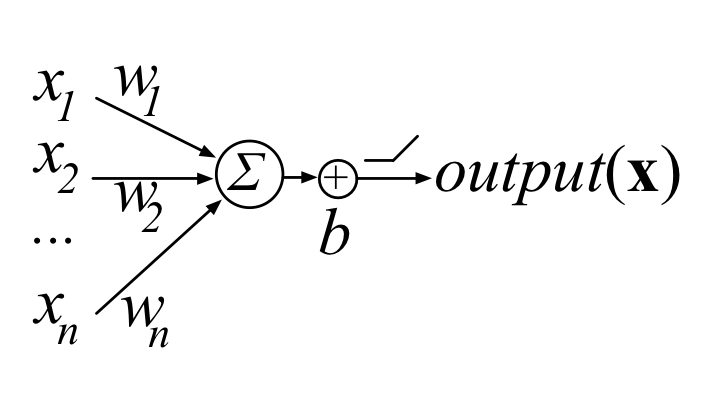
\includegraphics[scale=.9]{neuron.png}
\end{center}

Training this neuron means choosing weights $\mathbf{w}$ and bias $b$ so that we get the desired output for all inputs $\mathbf{x}$.  To do that, we minimize a {\em loss function} that compares $output({\mathbf{x}})$ with the desired output for all input $\mathbf{x}$ vectors. To minimize the loss function, we use some variation on gradient  descent, which requires the partial derivative (the gradient) of $output({\mathbf{x}})$ with respect to model parameters $\mathbf{w}$ and $b$. Our goal is to gradually tweak $\mathbf{w}$ and $b$ so that the overall loss function keeps getting smaller across all $\mathbf{x}$ inputs.

If we're careful, we can derive the gradient by differentiating the scalar version of a common loss function (mean squared error), $\frac{1}{n} \Sigma_{\mathbf{x}} ||desiredoutput(\mathbf{x}) - output(\mathbf{x})||_2^2 = \frac{1}{n} \Sigma_{\mathbf{x}} ||desiredoutput(\mathbf{x}) - max(0, \Sigma_i^n w_i x_i + b)||_2^2$. But this is just one neuron and full networks must train the weights and biases of all neurons simultaneously. We really need general rules for the derivative of a function with respect to a vector and even rules for the derivative of a vector-valued function with respect to a vector.

This article walks through the derivation of some important rules for computing partial derivatives with respect to vectors, particularly those useful for training neural networks. There are lots of useful resources on the net, such as https://www.math.uwaterloo.ca/~hwolkowi/matrixcookbook.pdf and  https://www.comp.nus.edu.sg/~cs5240/lecture/matrix-differentiation.pdf but they mainly provide results. In contrast, we're going to rederive and ``rediscover'' some key matrix calculus rules in an effort to explain them.

\section{Review: Scalar derivative rules}

It's probably a good idea to summarize the main scalar derivative rules just so we have everything in one place.

$
\begin{array}{lcc}
Rule & \text{Scalar function } f(x) & \text{Scalar derivative of $f(x)$ with respect to } x\\
\hline
\vspace{1mm}
\text{Multiplication by constant} &	cf	&c \frac{df}{dx}\\
\vspace{1mm}
\text{Power Rule}	& x^n	& nx^{n-1}\\
\vspace{1mm}
\text{Sum Rule}	& f + g	& \frac{df}{dx} + \frac{dg}{dx}\\
\vspace{1mm}
\text{Difference Rule}	& f - g	& \frac{df}{dx} - \frac{dg}{dx}\\
\vspace{1mm}
\text{Product Rule}	& fg & f \frac{dg}{dx} + \frac{df}{dx} g\\
\vspace{1mm}
\text{Quotient Rule}	& \frac{f}{g} = fg^{-1} & f \frac{dg}{dx}^{-1} + \frac{df}{dx} g^{-1}\\
\text{Chain Rule}	 & f(g(x)) &   \frac{df(g(x))}{dx}\frac{dg(x)}{dx}\\
\end{array}
$

When a function has a single parameter, $f(x)$, you'll often see $f'$ and $f'(x)$ used as shorthands for $\frac{d}{dx} f(x)$. We recommend against this notation as it does not make clear the variable we're taking the derivative with respect to.

You can think of $\frac{d}{dx}$ as an operator that maps a function of one parameter to another function. So to take the derivative with respect to $x$ of $cx$, $\frac{d}{dx} cx$, we are really just moving the constant to the left of the operator: $c\frac{d}{dx}x$ or $c\frac{dx}{dx}$, which makes it more clear that the derivative is $c \times 1 = c$.  We are used to this simplification for the usual arithmetic operators. For example, $-2x = 2 \times -x$ where the negation operator is analogous to our derivative operator. We have just moved to the scalar outside of the operation. Thinking of the derivative as an operator is handy when solving complicated derivatives as we can mechanically apply rules of differentiation.

\section{Review: Vector calculus and partial derivatives}

Real-world problems are rarely so simple that we can express them as a single function of a single parameter, $f(x)$. Let's move on to functions of multiple parameters such as $f(x,y)$. We compute derivatives with respect to one variable (parameter) at a time, giving us two different {\em partial derivatives} for this two-parameter function.  Instead of using operator $\frac{d}{dx}$, we use $\frac{\partial}{\partial x}$ (a stylized $d$ and not the Greek letter $\delta$). For functions of a single parameter, operator $\frac{\partial}{\partial x}$ is equivalent to $\frac{d}{dx}$ (for sufficiently smooth functions), but you should restrict your use of $\frac{d}{dx}$ to functions of a single parameter.

The partial derivative with respect to $x$ is just the usual scalar derivative but treating any other variable in the equation as a constant.  Consider function $f(x,y) = 3x^2y$. The partial derivative with respect to $x$ is written $\frac{\partial}{\partial x} 3x^2y$. There are three constants from the perspective of $\frac{\partial}{\partial x}$: 3, 2, and $y$. Therefore, $\frac{\partial}{\partial x} 3yx^2 = 3y\frac{\partial}{\partial x} x^2 = 3y2x = 6yx$. The partial derivative with respect to $y$ treats $x$ like a constant now: $\frac{\partial}{\partial y} 3x^2y = 3x^2\frac{\partial}{\partial y} y = 3x^2\frac{\partial y}{\partial y} = 3x^2 \times 1 = 3x^2$. 

So, partial derivatives use the usual scalar derivative rules while holding all but a single variable, $x$, as constants for the purpose of computing the partial derivative with respect to $x$.

To make it clear we are doing vector calculus and not just multivariate calculus, let's consider what we do with the partial derivatives $\frac{\partial f(x,y)}{\partial x}$ and $\frac{\partial f(x,y)}{\partial y}$ we computed for $f(x,y) = 3x^2y$. Currently they're just kind of floating around and not organized in any way so let's organize them into a horizontal vector. We call this vector the {\em gradient} of $f(x,y)$ and write it as:

$\nabla f(x,y)  = [ \frac{\partial f(x,y)}{\partial x} ~\frac{\partial f(x,y)}{\partial y}] = [6yx ~3x^2]$

Vector calculus deals with functions mapping $n$ real parameters to a real scalar, $f : \mathbb{R}^n \rightarrow \mathbb{R}$.  Now, let's get crazy and consider multiple functions simultaneously, $\mathbf{f}: \mathbb{R}^n \rightarrow \mathbb{R}^m$.

\section{Matrix calculus}

Moving from vector calculus to matrix calculus now, let's compute partial derivatives for two functions, both of which take two parameters.  We can keep the same $f(x,y)$ from the last section, but let's add $g(x,y) = 2x + y^8$.  The gradient for $g$ has two entries, a partial derivative for each parameter. The partials are:

$\frac{\partial g(x,y)}{\partial x} = \frac{\partial 2x}{\partial x} + \frac{\partial y^8}{\partial x} = 2\frac{\partial x}{\partial x} + 0 = 2 \times 1 = 1$

and

$\frac{\partial g(x,y)}{\partial y} = \frac{\partial 2x}{\partial y} + \frac{\partial y^8}{\partial y} = 0 + 8y^7 = 8y^7$

giving us gradient $\nabla g(x,y) = [1, 8y^7]$.

Gradient vectors organize all of the partial derivatives for a specific scalar function. If we have two functions, we can also organize their gradients into a matrix called the {\em Jacobian matrix} where the gradients are rows:

$J =
\begin{bmatrix}
	\nabla f(x,y)\\
	\nabla g(x,y)
\end{bmatrix} = \begin{bmatrix}
\frac{\partial f(x,y)}{\partial x} & \frac{\partial f(x,y)}{\partial y}\\
\frac{\partial g(x,y)}{\partial x} & \frac{\partial g(x,y)}{\partial y}\\
\end{bmatrix} = \begin{bmatrix}
	6yx & 3x^2\\
	1 & 8y^7
\end{bmatrix}
$

Welcome to matrix calculus!

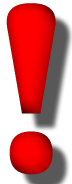
\includegraphics[scale=.08]{redbang.png} Before moving on, please note that there are multiple ways to represent the Jacobian. We are using the so-called [numerator layout](https://en.wikipedia.org/wiki/Matrix\_calculus\#Layout\_conventions) but many papers and software will use the transpose of this Jacobian (flip it around its diagonal).

\subsection{Generalization of the Jacobian}

So far, we've looked at a specific example of a Jacobian matrix. To define a Jacobian matrix, let's combine multiple parameters into a single vector argument: $f(x,y,z) \Rightarrow f(\mathbf{x})$. Lowercase letters in bold font such as $\mathbf{x}$ are vectors and math italics font like $x$ are scalars; $x_i$ is the $i{th}$ element of vector $\mathbf{x}$. We also have to define an orientation for vector $\mathbf{x}$. We'll assume that all vectors are vertical by default of size $n \times 1$:

$\mathbf{x} = \begin{bmatrix}
           x_1\\
           x_2\\
           \vdots \\
           x_n\\
           \end{bmatrix}$

With multiple scalar-valued functions, we can combine them all into a vector just like we did with the parameters. Let $\mathbf{y} = \mathbf{f}(\mathbf{x})$ be a vector of $m$ scalar-valued functions, $\mathbf{f}: \mathbb{R}^n \rightarrow \mathbb{R}^m$ with $n=|\mathbf{x}|$. Each $f_i$ function within $\mathbf{f}$  is a scalar, $f_i : R^n \rightarrow R$ like we had in the previous section:

$
\begin{array}{lcl}
y_1 & = & f_1(\mathbf{x})\\
y_2 & = & f_2(\mathbf{x})\\
 & \vdots & \\
y_m & = & f_m(\mathbf{x})\\
\end{array}
$

It's very often the case that $m=n$ because we will have a scalar function result for each element of the vector; this is the case for $\mathbf{y} = \mathbf{x}$, for example.

The Jacobian matrix is the collection of all $m \times n$ possible partial derivatives:

$
\frac{\partial \mathbf{y}}{\partial \mathbf{x}} = \begin{bmatrix}
\frac{\partial}{\partial \mathbf{x}} f_1(\mathbf{x}) \\
\frac{\partial}{\partial \mathbf{x}} f_2(\mathbf{x})\\
\ldots\\
\frac{\partial}{\partial \mathbf{x}} f_m(\mathbf{x})
\end{bmatrix}
$

where each $\frac{\partial}{\partial \mathbf{x}} f_i(\mathbf{x})$ is an $n$-vector because the partial derivative is with respect to a vector, $\mathbf{x}$, whose length is $n = |\mathbf{x}|$.  The width of the Jacobian is the length of the vector $\mathbf{x}$ if we're taking partial derivative with respect to $\mathbf{x}$.  The Jacobian is always $m$ rows for $n$ equations.  It helps to think about the Jacobian shapes visually:

\begin{center}
\begin{tabular}{c|ccl}
\parbox[b][40pt][c]{40pt}{Jacobian shape table}  & ~\framebox(25,25){$x$} & \framebox(25,60){$\mathbf{x}$}\\
\hline
\\[\dimexpr-\normalbaselineskip+5pt]
\framebox(25,25){$f$} &~\framebox(25,25){$\frac{\partial f}{\partial {x}}$} & \framebox(60,25){$\frac{\partial f}{\partial {\mathbf{x}}}$}&\\
\framebox(25,60){$\mathbf{f}$} &~\framebox(25,60){$\frac{\partial \mathbf{f}}{\partial {x}}$} & \framebox(60,60){$\frac{\partial \mathbf{f}}{\partial \mathbf{x}}$}\\
\end{tabular}
\end{center}

To represent the trivial equation $\mathbf{y} = \mathbf{x}$, for example, $f_i(\mathbf{x}) = x_i$. In this case, the Jacobian is the identity matrix since $m=n$ (a Jacobian matrix size $m \times n$ where $m = |\mathbf{f}| = n = |\mathbf{x}|$).

$
\begin{array}{lll}
\frac{\partial \mathbf{y}}{\partial \mathbf{x}} = \begin{bmatrix}
\frac{\partial}{\partial {x}} f_1(\mathbf{x}) \\
\frac{\partial}{\partial {x}} f_2(\mathbf{x})\\
\ldots\\
\frac{\partial}{\partial {x}} f_m(\mathbf{x})
\end{bmatrix} &=& \begin{bmatrix}
\frac{\partial}{\partial {x_1}} f_1(\mathbf{x})~ \frac{\partial}{\partial {x_2}} f_1(\mathbf{x}) ~\ldots~ \frac{\partial}{\partial {x_n}} f_1(\mathbf{x}) \\
\frac{\partial}{\partial {x_1}} f_2(\mathbf{x})~ \frac{\partial}{\partial {x_2}} f_2(\mathbf{x}) ~\ldots~ \frac{\partial}{\partial {x_n}} f_2(\mathbf{x}) \\
\ldots\\
~\frac{\partial}{\partial {x_1}} f_m(\mathbf{x})~ \frac{\partial}{\partial {x_2}} f_m(\mathbf{x}) ~\ldots~ \frac{\partial}{\partial {x_n}} f_m(\mathbf{x}) \\
\end{bmatrix}\\\\
 & = & \begin{bmatrix}
\frac{\partial}{\partial {x_1}} x_1~ \frac{\partial}{\partial {x_2}} x_1 ~\ldots~ \frac{\partial}{\partial {x_n}} x_1 \\
\frac{\partial}{\partial {x_1}} x_2~ \frac{\partial}{\partial {x_2}} x_2 ~\ldots~ \frac{\partial}{\partial {x_n}} x_2 \\
\ldots\\
~\frac{\partial}{\partial {x_1}} x_m~ \frac{\partial}{\partial {x_2}} x_m ~\ldots~ \frac{\partial}{\partial {x_n}} x_m \\
\end{bmatrix}\\\\
& & (\text{and since } \frac{\partial}{\partial {x_j}} x_i = 0 \text{ for } j \neq i)\\\\
 & = & \begin{bmatrix}
\frac{\partial}{\partial {x_1}} x_1 & 0 & \ldots& 0 \\
0 & \frac{\partial}{\partial {x_2}} x_2 &\ldots & 0 \\
& & \ddots\\
0 & 0 &\ldots& \frac{\partial}{\partial {x_n}} x_m \\
\end{bmatrix}\\\\
 & = & \begin{bmatrix}
1 & 0 & \ldots& 0 \\
0 &1 &\ldots & 0 \\
& & \ddots\\
0 & 0 & &1 \\
\end{bmatrix}\\\\
& = & I\\
\end{array}
$

It's very important to track whether a matrix is vertical or horizontal, $\mathbf{x}$ or $\mathbf{x}^T$. Also make sure you pay attention to whether something is a scalar-valued function or a vector valued function. Is it $\mathbf{y} = \ldots$ or $y = \ldots$?

When trying to deduce the Jacobian of a complex vector equation, a good trick is to reduce everything down to a set of scalar equations and then take all of the partials derivatives, combining the results appropriately into vectors and matrices.

\subsection{Derivatives of vector element-wise binary operators}

Element-wise binary operations on vectors, such as vector addition $\mathbf{w} + \mathbf{x}$, are important because we can express many common vector operations, such as vector-constant-scalar multiplication, as element-wise binary operations.  We can generalize the element-wise binary operations with notation $\mathbf{y} = \mathbf{f(w)} \bigcirc \mathbf{g(x)}$ where $m=n=|y|=|w|=|x|$. The $\bigcirc$ symbol represents any element-wise operator and not the $\circ$ function composition operator.  Here's what that equation looks like when we zoom in to examine the scalar equations:

$\begin{bmatrix}
           y_1\\
           y_2\\
           \vdots \\
           y_n\\
           \end{bmatrix} = \begin{bmatrix}
           f_{1}(\mathbf{w}) \bigcirc g_{1}(\mathbf{x})\\
           f_{n}(\mathbf{w}) \bigcirc g_{2}(\mathbf{x})\\
           \vdots \\
           f_{n}(\mathbf{w}) \bigcirc g_{n}(\mathbf{x})\\
         \end{bmatrix}$

where we write $n$ not $m$ equations vertically to emphasize the fact that the result of element-wise operators give $m=n$ sized vector results.

The general case for the Jacobian with respect to $\mathbf{w}$ is the square matrix:

$
\frac{\partial \mathbf{y}}{\partial \mathbf{w}}  = \begin{bmatrix}
\frac{\partial}{\partial w_1} ( f_{1}(\mathbf{w}) \bigcirc g_{1}(\mathbf{x}) ) & \frac{\partial}{\partial w_2} ( f_{1}(\mathbf{w}) \bigcirc g_{1}(\mathbf{x}) ) & \ldots & \frac{\partial}{\partial w_n} ( f_{1}(\mathbf{w}) \bigcirc g_{1}(\mathbf{x}) )\\\\
\frac{\partial}{\partial w_1} ( f_{2}(\mathbf{w}) \bigcirc g_{2}(\mathbf{x}) ) & \frac{\partial}{\partial w_2} ( f_{2}(\mathbf{w}) \bigcirc g_{2}(\mathbf{x}) ) & \ldots & \frac{\partial}{\partial w_n} ( f_{2}(\mathbf{w}) \bigcirc g_{2}(\mathbf{x}) )\\\\
& \ldots\\\\
\frac{\partial}{\partial w_1} ( f_{n}(\mathbf{w}) \bigcirc g_{n}(\mathbf{x}) ) & \frac{\partial}{\partial w_2} ( f_{n}(\mathbf{w}) \bigcirc g_{n}(\mathbf{x}) ) & \ldots & \frac{\partial}{\partial w_n} ( f_{n}(\mathbf{w}) \bigcirc g_{n}(\mathbf{x}) )\\
\end{bmatrix}
$

and the Jacobian with respect to $\mathbf{x}$:

$
\frac{\partial \mathbf{y}}{\partial \mathbf{x}}  = \begin{bmatrix}
\frac{\partial}{\partial x_1} ( f_{1}(\mathbf{w}) \bigcirc g_{1}(\mathbf{x}) ) & \frac{\partial}{\partial x_2} ( f_{1}(\mathbf{w}) \bigcirc g_{1}(\mathbf{x}) ) & \ldots & \frac{\partial}{\partial x_n} ( f_{1}(\mathbf{w}) \bigcirc g_{1}(\mathbf{x}) )\\\\
\frac{\partial}{\partial x_1} ( f_{2}(\mathbf{w}) \bigcirc g_{2}(\mathbf{x}) ) & \frac{\partial}{\partial x_2} ( f_{2}(\mathbf{w}) \bigcirc g_{2}(\mathbf{x}) ) & \ldots & \frac{\partial}{\partial x_n} ( f_{2}(\mathbf{w}) \bigcirc g_{2}(\mathbf{x}) )\\\\
& \ldots\\\\
\frac{\partial}{\partial x_1} ( f_{n}(\mathbf{w}) \bigcirc g_{n}(\mathbf{x}) ) & \frac{\partial}{\partial x_2} ( f_{n}(\mathbf{w}) \bigcirc g_{n}(\mathbf{x}) ) & \ldots & \frac{\partial}{\partial x_n} ( f_{n}(\mathbf{w}) \bigcirc g_{n}(\mathbf{x}) )\\
\end{bmatrix}
$

That's quite a furball, but the Jacobian is very commonly a diagonal matrix, a matrix that is zero everywhere but the diagonal. 

If $f_i(\mathbf{w})$ and $g_i(\mathbf{x})$ are purely functions of at most $w_i$ and $x_i$, respectively, and no other elements of vector $\mathbf{w}$ or $\mathbf{x}$, we can reduce $f_i(\mathbf{w}) \bigcirc g_i(\mathbf{x})$ to $f_i(w_i) \bigcirc g_i(x_i)$. This is technically an abuse of our notation because $f_i$ and $g_i$ are functions of vectors not individual elements. We should really write something like $\hat f_{i}(w_i) = f_{i}(\mathbf{w})$, but that would muddy the equations further (and programmers are comfortable overloading functions) so we'll proceed with the notation anyway.

With the constraint that $f_i(\mathbf{w})$ and $g_i(\mathbf{x})$ can only access $w_i$ and $x_i$, the elements along the diagonal of the Jacobian are $\frac{\partial}{\partial x_i} ( f_i(w_i) \bigcirc g_i(x_i) )$:

$
\frac{\partial \mathbf{y}}{\partial \mathbf{w}}  = \begin{bmatrix}
\frac{\partial}{\partial w_1} ( f_{1}(w_1) \bigcirc g_{1}(x_1) )\\
& \frac{\partial}{\partial w_2} (f_{2}(w_2) \bigcirc g_{2}(x_2) ) & &\text{\huge0}\\
& & \ldots \\
\text{\huge0}& & & \frac{\partial}{\partial w_n} (f_{n}(w_n) \bigcirc g_{n}(x_n) )
\end{bmatrix}
$

Or more succinctly,

$\frac{\partial \mathbf{y}}{\partial \mathbf{w}} = diag \left( \frac{\partial}{\partial w_1}(f_{1}(w_1) \bigcirc g_{1}(x_1)),~ \frac{\partial}{\partial w_2}(f_{2}(w_2) \bigcirc g_{2}(x_2)),~ \ldots,~ \frac{\partial}{\partial w_n}(f_{n}(w_n) \bigcirc g_{n}(x_n)) \right)$

and

$\frac{\partial \mathbf{y}}{\partial \mathbf{x}} = diag \left( \frac{\partial}{\partial x_1}(f_{1}(w_1) \bigcirc g_{1}(x_1)),~ \frac{\partial}{\partial x_2}(f_{2}(w_2) \bigcirc g_{2}(x_2)),~ \ldots,~ \frac{\partial}{\partial x_n}(f_{n}(w_n) \bigcirc g_{n}(x_n)) \right)$

where $diag(\mathbf{x})$ constructs a matrix whose diagonal elements are taken from vector $\mathbf{x}$: $diag(\mathbf{x}) = \mathbf{x}^T I$.

We know that all off-diagonal entries are 0 because for $j \neq i$:

$\frac{\partial}{\partial w_j} ( f_i(w_i) \bigcirc g_i(x_i) ) = \frac{\partial}{\partial x_j} ( f_i(w_i) \bigcirc g_i(x_i) ) = 0$

When $j \neq i$, $f_i(w_i) \bigcirc g_i(x_i)$ looks like a constant to the partial derivative operators $\frac{\partial}{\partial w_j}$ and $\frac{\partial}{\partial x_j}$, and the derivative of any constant is 0.

Because we do lots of simple vector arithmetic, the general function $\mathbf{f(w)}$ is often just the vector $\mathbf{w}$.  Any time the general function is a vector, we know that $f_i(\mathbf{w})$ reduces to $f_i(w_i) = w_i$. For example, vector addition $\mathbf{w + x}$ fits our general case as $\mathbf{f(w)} + \mathbf{g(x)}$ with scalar equations $y_i = f_i(\mathbf{w}) + g_i(\mathbf{x})$. But, that reduces to just $y_i = f_i(w_i) + g_i(x_i) = w_i + x_i$ and so we get partial derivatives:

$\frac{\partial}{\partial w_i} ( f_{i}(w_i) + g_{i}(x_i) ) = \frac{\partial}{\partial w_i}(w_i + x_i) = 1 + 0 = 1$\\
$\frac{\partial}{\partial x_i} ( f_{i}(w_i) + g_{i}(x_i) ) = \frac{\partial}{\partial x_i}(w_i + x_i) = 0 + 1 = 1$


That gives us $\frac{\partial (\mathbf{w+x})}{\partial \mathbf{w}} = \frac{\partial (\mathbf{w+x})}{\partial \mathbf{x}} = I$, the identity matrix, because every element along the diagonal is 1.

Given the simplicity of this special case, $f_i(\mathbf{w})$ reducing to $f_i(w_i)$, we can easily write out the Jacobian's for the common element-wise binary operations on vectors:

$
\begin{array}{lllll}
\text{Op} & \text{Partial with respect to } \mathbf{w} & \text{Partial with respect to }\mathbf{x}\\
\hline\\

+ & \frac{\partial (\mathbf{w+x})}{\partial \mathbf{w}} = diag(\ldots \frac{\partial (w_i + x_i)}{\partial w_i} \ldots) = diag(\vec{1}) = I & \frac{\partial (\mathbf{w+x})}{\partial \mathbf{x}} =  I\\\\

- & \frac{\partial (\mathbf{w-x})}{\partial \mathbf{w}}  =  diag(\ldots\frac{\partial (w_i - x_i)}{\partial w_i}\ldots) =  diag(\vec{1})  =  I & \frac{\partial (\mathbf{w-x})}{\partial \mathbf{x}}  =  diag(\ldots\frac{\partial (w_i - x_i)}{\partial x_i}\ldots)  =  diag(-\vec{1})  =  -I \\\\

\otimes & \frac{\partial (\mathbf{w \otimes x})}{\partial \mathbf{w}}  =  diag(\ldots\frac{\partial (w_i \times x_i)}{\partial w_i} \ldots)  =  diag(\mathbf{x}) & \frac{\partial (\mathbf{w \otimes x})}{\partial \mathbf{x}}  =  diag(\mathbf{w})\\\\

\oslash & \frac{\partial (\mathbf{w \oslash x})}{\partial \mathbf{w}}  =  diag(\ldots\frac{\partial (w_i / x_i)}{\partial w_i}\ldots)  =  diag(\ldots \frac{1}{x_i} \ldots) & \frac{\partial (\mathbf{w \oslash x})}{\partial \mathbf{x}}  =  diag(\ldots \frac{-w_i}{x_i^2} \ldots)\\

\end{array}
$

The $\otimes$ and $\oslash$ operators are element-wise multiplication and division; $\otimes$ is sometimes called the {\em Hadamard product}.

\subsection{Derivatives involving scalar expansion}

When we add or multiply scalars to vectors, we are implicitly expanding the scalar to a vector and then performing an element-wise operation. For example, adding scalar $z$  to vector $\mathbf{x}$, $\mathbf{y} = \mathbf{x} + z$,
is really
$\mathbf{y} = \mathbf{f(x)} + \mathbf{g}(z)$ where $\mathbf{f(x)} = \mathbf{x}$ and $\mathbf{g}(z) = \vec{1} z$.  It's okay to think of variable $z$ as a constant for our discussion here, but $z$ is more generally a scalar that doesn't depend on $\mathbf{x}$. We need this condition so that $\frac{\partial z}{\partial x_i} = 0$ for any $x_i$.
Similarly, multiplying by a scalar, $\mathbf{y} = \mathbf{x} z$,
is really
$\mathbf{y} = \mathbf{f(x)} \otimes \mathbf{g}(z)$ where $\otimes$ is the element-wise  multiplication (Hadamard product) of the two vectors.

The partial derivative of vector-scalar addition and multiplication with respect to vector $\mathbf{x}$ fall out from our element-wise rule:

$\frac{\partial \mathbf{y}}{\partial \mathbf{x}} = diag \left( \ldots \frac{\partial}{\partial x_i} ( f_i(x_i) \bigcirc g_i(z) ) \ldots \right)$

since we've identified $f_i(x_i) = x_i$ and $g_i(z) = z$ where $z$ doesn't depend on $\mathbf{x}$. Note that functions $\mathbf{f(x)} = \mathbf{x}$ and $\mathbf{g}(z) = \vec{1} z$ clearly satisfy our constraint for the special case of diagonal Jacobian (that $f_i(\mathbf{x})$ refer at most to $x_i$ and $g_i(z)$ refers to the $i^{th}$ value of the $\vec{1}z$ vector where $z$ doesn't depend on $\mathbf{x}$). 

Using the usual rules for scalar partial derivatives, we arrive at the following diagonal elements of the Jacobian for vector-scalar addition:
 
$\frac{\partial}{\partial x_i} ( f_i(x_i) + g_i(z) ) = \frac{\partial (x_i + z)}{\partial x_i} = \frac{\partial x_i}{\partial x_i} + \frac{\partial z}{\partial x_i} = 1 + 0 = 1$

So, $\frac{\partial}{\partial \mathbf{x}} ( \mathbf{x} + z ) = diag(\vec{1}) = I$.

Computing the partial derivative with respect to the single-valued parameter $z$, however, results in a vertical vector not a diagonal matrix whose elements are:
 
$\frac{\partial}{\partial z} ( f_i(x_i) + g_i(z) ) = \frac{\partial (x_i + z)}{\partial z} = \frac{\partial x_i}{\partial z} + \frac{\partial z}{\partial z} = 0 + 1 = 1$

Therefore, $\frac{\partial}{\partial z} ( \mathbf{x} + z ) = \vec{1}$.

The diagonal elements of the Jacobian for vector-scalar multiplication involve the product rule for scalar derivatives:

$\frac{\partial}{\partial x_i} ( f_i(x_i) \otimes g_i(z) ) = x_i  \frac{\partial z}{\partial x_i} + z  \frac{\partial x_i}{\partial x_i} = 0 + z = z$

So, $\frac{\partial}{\partial \mathbf{x}} ( \mathbf{x} z ) = diag(\vec{1}  z) = I z$. 

The partial derivative with respect to single-valued parameter $z$ is a vertical vector whose elements are:

$\frac{\partial}{\partial z} ( f_i(x_i) \otimes g_i(z) ) = x_i \frac{\partial z}{\partial z} + z \frac{\partial x_i}{\partial z} = x_i + 0 = x_i$

This gives us $\frac{\partial}{\partial z} ( \mathbf{x}s z ) = \mathbf{x}$.

\subsection{Vector sum}

Summing the elements of a vector is an important operation in and of itself in applications based upon linear algebra, such as the neuron output function, but we can also use it as a way to simplify computing the derivative of vector dot product and other operations that reduce vectors to scalars.

Let $y = sum( \mathbf{f}(\mathbf{x})) = \Sigma_{i=1}^n f_i(\mathbf{x})$ where we have to be careful to leave the parameter as a vector $\mathbf{x}$ because each function $f_i$ could use all values in the vector not just $x_i$. The sum is over the {\bf results} of the function and not the parameter. The gradient ($1 \times n$ Jacobian) of vector summation is:

$
\begin{array}{lcl}
\frac{\partial y}{\partial \mathbf{x}} & = & \begin{bmatrix} \frac{\partial y}{\partial x_1}, \frac{\partial y}{\partial x_2}, \ldots, \frac{\partial y}{\partial x_n} \end{bmatrix}\\\\
 & = & \begin{bmatrix} \frac{\partial}{\partial x_1} \Sigma_i f_i(\mathbf{x}),~ \frac{\partial}{\partial x_2} \Sigma_i f_i(\mathbf{x}),~ \ldots,~ \frac{\partial}{\partial x_n} \Sigma_i  f_i(\mathbf{x}) \end{bmatrix} \\\\
 & = & \begin{bmatrix} \Sigma_i \frac{\partial f_i(\mathbf{x})}{\partial x_1},~ \Sigma_i \frac{\partial f_i(\mathbf{x})}{\partial x_2},~ \ldots,~ \Sigma_i \frac{\partial f_i(\mathbf{x})}{\partial x_n}  \end{bmatrix}(\text{move derivative inside }\Sigma)\\\\
\end{array}
$

The summation inside the gradient elements can be tricky so make sure to keep your notation consistent. 

Let's look at the gradient of the simple $y = sum(\mathbf{x})$. The function inside the summation is just $f_i(\mathbf{x}) = x_i$ and the gradient is then:

$\nabla y = \begin{bmatrix} \Sigma_i \frac{\partial f_i(\mathbf{x})}{\partial x_1},~ \Sigma_i \frac{\partial f_i(\mathbf{x})}{\partial x_2},~ \ldots,~ \Sigma_i \frac{\partial f_i(\mathbf{x})}{\partial x_n}  \end{bmatrix} = \begin{bmatrix} \Sigma_i \frac{\partial x_i}{\partial x_1},~ \Sigma_i \frac{\partial x_i}{\partial x_2},~ \ldots,~ \Sigma_i \frac{\partial x_i}{\partial x_n}  \end{bmatrix}$

Because $\frac{\partial}{\partial x_j} x_i = 0$ for $j \neq i$, we can simplify to:

$\nabla y = \begin{bmatrix} \frac{\partial x_1}{\partial x_1},~ \frac{\partial x_2}{\partial x_2},~ \ldots,~ \frac{\partial x_n}{\partial x_n}  \end{bmatrix} = \begin{bmatrix}1, 1, \ldots, 1\end{bmatrix} = \vec{1}^T$

Notice that the result is a horizontal vector full of 1s, not a vertical vector, and so the gradient is $\vec{1}^T$. It's very important to keep the shape of all of your vectors and matrices in order otherwise it's impossible to compute the derivatives of complex functions.

As another example, let's sum the result of multiplying a vector by a constant scalar.  If $y = sum(\mathbf{x} z)$ then $f_i(\mathbf{x},z) = x_i z$. The gradient is:

$
\begin{array}{lcl}
\frac{\partial y}{\partial \mathbf{x}} & = & \begin{bmatrix} \Sigma_i \frac{\partial}{\partial x_1} x_i z,~ \Sigma_i \frac{\partial }{\partial x_2} x_i z,~ \ldots,~ \Sigma_i \frac{\partial}{\partial x_n} x_i z  \end{bmatrix}\\\\
 & = & \begin{bmatrix} \frac{\partial}{\partial x_1} x_1 z,~ \frac{\partial }{\partial x_2} x_2 z,~ \ldots,~ \frac{\partial}{\partial x_n} x_n z  \end{bmatrix}\\\\
 & = & \begin{bmatrix} z, z, \ldots, z \end{bmatrix}\\\\
\end{array}
$

The derivative with respect to scalar variable $z$ is $1 \times 1$:

$
\begin{array}{lcl}
\frac{\partial y}{\partial z} & = & \frac{\partial}{\partial z} \Sigma_{i=1}^n (x_i+z)\\\\
& = & \Sigma_i \frac{\partial}{\partial z} (x_i+z)\\\\
& = & \Sigma_i (0 + 1)\\\\
& = & n
\end{array}
$

\subsection{Vector chain rule}

We can't compute partial derivatives of very complicated functions using just the basic matrix calculus rules we've seen so far. We need to be able to combine them using the so-called {\em chain rule}.  The chain rule is a divide and conquer strategy (like Quicksort) that breaks complicated expressions into subexpressions that are easier to compute derivatives for.  The chain rule comes into play when we need the derivative of an expression with nested subexpressions, such as $\frac{d}{dx} sin(x^2)$.  

In general, the chain rule is defined in terms of expressions that can be written as $y = f(g(x))$. (You will also see the chain rule defined using function composition $(f \circ g)(x)$ which is the same thing.)  Some sources write the derivative using shorthand notation $f'(g(x))g'(x)$, but that hides the fact that we are performing a variable substitution: $u = g(x)$. It's better to define the chain rule explicitly via the following so we never take the derivative with respect to the wrong variable.

$\frac{dy}{dx} = \frac{dy}{du} \frac{du}{dx}$.

In this case, we split $sin(x^2)$ into two functions:

$u = g(x) = x^2$\\
$y = f(u) = sin(u)$

Putting the functions $f$ and $g$ and their parameters in there makes it clear which variables we must take the derivative with respect to. The order of these subexpressions does not affect the answer, but we recommend working in the reverse order of operations dictated by the nesting (innermost to outermost). That way, expressions and derivatives are always functions of previously-computed elements. Here are the derivatives of the simplified functions:

$\frac{du}{dx} = \frac{d}{dx} x^2 = 2x$\\
$\frac{dy}{du} = \frac{d}{du} sin(u) = cos(u)$

Now, we just have to combine the derivatives using the chain rule, which means multiplying the two derivatives together:

$\frac{dy}{dx} = \frac{dy}{du} \frac{du}{dx} = cos(u) 2x$

then substituting the intermediate variable back in

$\frac{dy}{dx} = cos(x^2) 2x = 2xcos(x^2)$

You can think of the chain rule in terms of units canceling. If we let $y$ be gallons of gas, $x$ be the gallons in a gas tank, and $u$ as miles we can interpret $\frac{dy}{dx}$ as $\frac{miles}{tank} = \frac{miles}{gallon} \frac{gallon}{tank}$. The $gallon$ denominator and numerator cancel. This is a convenient way to remember the chain rule but the analogy only goes so far; don't treat $dy$ and $dx$ has separate variables since they are two components in the name of a single operator.

When there is only one variable substitution, it's straightforward to directly write the derivative down without explicitly creating and substituting a temporary variable. With deeply nested expressions, however, it's easy to get lost and it's better to carefully track all of the intermediate variables.

It might help to think about deploying the chain rule the way a compiler implementor thinks about generating code for complicated expressions.  The compiler must unravel function call nesting like $f_1(f_2(f_3(f_4(x))))$ into a sequence of calls. The result of calling function $f_i$ is saved to a temporary variable called a register, which is then passed as a parameter to $f_{i-1}$.  Consider a nested equation like $y = f(x) = ln(sin(x^3)^2)$ that breaks down into subexpressions assigned to  intermediate (temporary) variables:

$r_1 = f_1(x) = x^3$\\
$r_2 = f_2(r_1) = sin(r_1)$\\
$r_3 = f_3(r_2) = r_2^2$\\
$r_4 = f_4(r_3) = ln(r_3)$ ~~~~~~($y = r_4$)

To compute the scalar derivative $\frac{dy}{dx}$, we can treat each of those subexpressions in isolation using just the basic scalar derivative rules.

$
\begin{array}{lllll}
\vspace{1mm}
\frac{d}{r_x} r_1 & = & \frac{d}{x} x^3 & = & 3x^2\\
\vspace{1mm}
\frac{d}{r_1} r_2 & = & \frac{d}{r_1} sin(r_1) & = & cos(r_1) \\
\frac{d}{r_2} r_3 & = & \frac{d}{r_2} r_2^2 & =& 2r_2\\
\frac{d}{r_3} r_4 & = & \frac{d}{r_3} ln(r_3) & =& \frac{1}{r_3}\\
\end{array}
$

Using the chain rule for 4 intermediate variables,

$\frac{dy}{dx} = \frac{dy}{r_4} \frac{d r_4}{r_3} \frac{dr_3}{d r_2} \frac{dr_2}{dr_1} \frac{dr_1}{dx}$

we get

$\frac{dy}{dx} = 1  \frac{1}{r_3}  2r_2  cos(r_1)  3x^2 = \frac{6r_2x^2cos(r_1)}{r_3}$

Substituting the intermediate variables back in, gives us:

$\frac{dy}{dx} = \frac{6sin(r_1)x^2cos(x^3)}{r_2^2} = \frac{6sin(x^3)x^2cos(x^3)}{sin(r_1)^2} = \frac{6sin(x^3)x^2cos(x^3)}{sin(x^3)^2} = \frac{6x^2cos(x^3)}{sin(x^3)}$

Ok, so much for the scalar chain rule. It turns out that the chain rule also works for computing partial derivatives of vector functions with respect to vectors.  Previously, we manually computed the derivative with respect to $\mathbf{x}$ of $y = sum(\mathbf{x}  z)$ as $[z, z, \ldots, z]$, but we can also use the chain rule. Let vector $\mathbf{u} = \mathbf{x}  z$ then $y = sum(\mathbf{u})$. The vector chain rule tells us that $\frac{dy}{d\mathbf{x}} = \frac{dy}{d\mathbf{u}}  \frac{d\mathbf{u}}{d\mathbf{x}}$, which means 

$\frac{dy}{d\mathbf{x}} = \vec{1}^T  \frac{d}{d\mathbf{x}} (\mathbf{x}  z) = \vec{1}^T  diag(\vec{1}z) = \vec{1}^T  I  z = \vec{1}^T  z = [z, z, \ldots, z]$

\subsection{Derivatives of vector dot product}

Now that we've got the chain rule in mind and we can compute the Jacobians for both element-wise binary operations and vector summation, we can define the gradient of the important vector dot product $y = \mathbf{f(w)} \cdot \mathbf{g(x)}$. (Note we use $y$ not $\mathbf{y}$ as the result is a scalar not a vector.) You will find the derivative of dot product defined as $f(\mathbf{x}) \cdot g'(\mathbf{x}) + f'(\mathbf{x}) \cdot g(\mathbf{x})$, but we'll use the chain rule instead to avoid having to memorize yet another rule.

Notice that dot product $\mathbf{w} \cdot \mathbf{x}$, such as we used in the neuron output function, is just the summation of the element-wise multiplication of the elements: $\Sigma_i^n (w_i x_i) = sum(\mathbf{w} \otimes \mathbf{x})$. (You might also find it useful to remember the linear algebra notation $\mathbf{w} \cdot \mathbf{x} = \mathbf{w}^{T} \times \mathbf{x}$.)  To use the chain rule, we perform a quick substitution, $\mathbf{u} = \mathbf{w} \otimes \mathbf{x}$ and $y = sum(\mathbf{u})$, and multiply their partial derivatives:

$\frac{d \mathbf{u}}{d\mathbf{x}} = \frac{d}{d\mathbf{x}} (\mathbf{w} \otimes \mathbf{x}) = diag(\mathbf{w})$\\
$\frac{dy}{d\mathbf{u}} = \frac{d}{d\mathbf{u}} sum(\mathbf{u}) = \vec{1}^T$

$\frac{dy}{d\mathbf{x}} = \frac{dy}{d\mathbf{u}} \times \frac{d\mathbf{u}}{d\mathbf{x}} = \vec{1}^T \times diag(\mathbf{w}) = \mathbf{w}^T$

Similarly, $\frac{dy}{d\mathbf{w}} = \mathbf{x}^T$. Note: the gradient is a horizontal vector (1 output)!

To check our results, we can also grind the dot product down into a pure scalar function:

$y = \mathbf{w} \cdot \mathbf{x} = \Sigma_i^n (w_i x_i)$

$\frac{\partial y}{\partial w_j} = \frac{\partial}{\partial w_j} \Sigma_i (w_i x_i) = \Sigma_i \frac{\partial}{\partial w_j} (w_i x_i) = \frac{\partial}{\partial w_j} (w_j x_j) = x_j$

Then:

$\frac{\partial y}{\partial \mathbf{w}} = [ x_1, \ldots, x_n ] = \mathbf{x}^T$

Our results match. 

\section{The punchline}

To train a neuron requires that we take the derivative of our loss  or ``cost'' function $C(\mathbf{w},b) = \frac{1}{n} \Sigma_{\mathbf{x}} ||desiredoutput(\mathbf{x}) - output(\mathbf{x})||_2^2$, with respect to the parameters of our model, $\mathbf{w}$ and $b$.  We won't solve that full problem here but we can apply the rules we've learned to compute partial derivatives of the weighted input to the rectified linear activation function, $z = \mathbf{w} \cdot \mathbf{x} + b$. The partial derivatives are:

$\frac{\partial z}{\partial \mathbf{w}} = \frac{\partial \mathbf{w} \cdot \mathbf{x}}{\partial \mathbf{w}} + \frac{\partial b}{\partial \mathbf{w}} = \mathbf{x}^T + \vec{0}^T = \mathbf{x}^T$

and

$\frac{\partial z}{\partial b} = \frac{\partial \mathbf{w} \cdot \mathbf{x}}{\partial b} + \frac{\partial b}{\partial b} = 0 + 1 = 1$

While we're at it, we can easily take the partials of the entire output function:
 
$output({\mathbf{x}}) = max(0, \mathbf{w} \cdot \mathbf{x} + b)$

The $max(0,z)$ function just says to treat all negative $z$ values as 0, so its derivative is 0 for $z \leq 0$ and $dz/dz = 1$ for $z > 0$. Because $output(\mathbf{x})$ is a nested function, we need the chain rule so let's use $z = \mathbf{w} \cdot \mathbf{x} + b$ to get $output(\mathbf{x}) = max(0,z(\mathbf{x}))$. Then,

$\frac{\partial output}{\partial \mathbf{w}} = \frac{\partial output}{\partial z}\frac{\partial z}{\partial \mathbf{w}}$

where

$\frac{\partial}{\partial z} output(\mathbf{x}) = \frac{\partial}{\partial z} max(z(\mathbf{x})) = \begin{cases}
	0 & z \leq 0\\
	1 & z > 0\\
\end{cases}
$

and, using $\frac{\partial z}{\partial \mathbf{w}} = \mathbf{x}^T$,

$\frac{\partial output}{\partial \mathbf{w}} = \begin{cases}
	0 & z \leq 0\\
	\mathbf{x}^T & z > 0\\
\end{cases}
$

Substituting $z = \mathbf{w} \cdot \mathbf{x} + b$, we get:

$\frac{\partial output}{\partial \mathbf{w}} = \begin{cases}
	\vec{0}^T & \mathbf{w} \cdot \mathbf{x} + b \leq 0\\
	\mathbf{x}^T & \mathbf{w} \cdot \mathbf{x} + b > 0\\
\end{cases}
$

which matches our intuition. The change in output when $z \leq 0$ is 0 for any $w_i$ change and the change in output is $x_i$ when $z > 0$ for any $w_i$ change. When $z > 0$, it's as if the $max$ function disappears. 

Turning to the partial with respect to $b$ now, we can use our intuition to jump directly to

$\frac{\partial output}{\partial b} = \begin{cases}
	0 & \mathbf{w} \cdot \mathbf{x} + b \leq 0\\
	\frac{\partial output}{\partial b} = 1 & \mathbf{w} \cdot \mathbf{x} + b > 0\\
\end{cases}
$

\section{Acknowledgements}

We thank [Yannet Interian](https://www.usfca.edu/faculty/yannet-interian) (Faculty in MS data science program at University of San Francisco) and [David Uminsky](http://www.cs.usfca.edu/~duminsky/) (Faculty/director of MS data science) for their help with the notation presented here..

\end{document}
